\documentclass[11pt,a4paper]{article}
\usepackage[
    left=0.73in,
    right=0.73in,
    top=.8in,
    bottom=.50in,
    paperheight=11in,
    paperwidth=8.5in
]{geometry}

\usepackage{array}
\newcolumntype{C}[1]{>{\centering\let\newline\\\arraybackslash\hspace{0pt}}m{#1}}
\usepackage{graphicx}
\usepackage{float}

\begin{document}
% Cover Page
\pagenumbering{gobble}
\begin{center}
\textbf{
    \Large{ECE 543: Introduction to Digital Systems}
    \\~\\
    \large{Instructor: Bessam Zuhair Al Jewad, Ph.D.}
    \\[1.25in]
    \LARGE{Prelab \#5: Combinational Logic Design}
    \\[0.62in]
    \large{Prepared for Himadri Basu (TA)\\~\\By Christopher Chin}
    \\[1.25in]
    \LARGE{Section 6}
    \\[1.25in]
    \Large{Department of Electrical and Computer Engineering\\
           University of New Hampshire}
    \\[1.25in]
    \Large{\today}
}
\end{center}
\clearpage
\pagenumbering{arabic}

% TOC
\tableofcontents
\pagebreak

% Pages
\section{Introduction}
\section{Equipment Required}
\begin{itemize}
    \item Global Specialties Design and Prototyping PB-505
    \item Wire leads
    \item Logic Probe (1)
    \item Seven-Segment LED Display (1)
    \item 7400 TTL NAND Integrated Circuit (2)
    \item 7410 TTL 3-Input NAND Integrated Circuit (3)
    \item 7404 TTL Inverter Integrated Circuit (1)
\end{itemize}
\section{Procedure}
\subsection{Binary to Octal Conversion Table}
\begin{tabular}{| C{1.2cm} | C{1.2cm} | C{1.2cm} || C{1.2cm} | C{1.2cm} | C{1.2cm} | C{1.2cm} | C{1.2cm} | C{1.2cm} | C{1.2cm} |}
    \hline
        \multicolumn{3}{|c|}{Inputs} &
        \multicolumn{7}{|c|}{Outputs} \\
    \hline $S_2$ & $S_1$ & $S_0$ & a & b & c & d & e & f & g \\
    \hline 0 & 0 & 0 & 0 & 0 & 0 & 0 & 0 & 0 & 1 \\
    \hline 0 & 0 & 1 & 1 & 0 & 0 & 1 & 1 & 1 & 1 \\
    \hline 0 & 1 & 0 & 0 & 0 & 1 & 0 & 0 & 1 & 0 \\
    \hline 0 & 1 & 1 & 0 & 0 & 0 & 0 & 1 & 1 & 0 \\
    \hline 1 & 0 & 0 & 1 & 0 & 0 & 1 & 1 & 0 & 0 \\
    \hline 1 & 0 & 1 & 0 & 1 & 0 & 0 & 1 & 0 & 0 \\
    \hline 1 & 1 & 0 & 0 & 1 & 0 & 0 & 0 & 0 & 0 \\
    \hline 1 & 1 & 1 & 0 & 0 & 0 & 1 & 1 & 1 & 1 \\
    \hline
\end{tabular}
\subsection{Truth Tables}
\subsection{K-maps}
\begin{tabular}{C{1.2cm} | C{1.2cm} | C{1.2cm} | C{1.2cm} | C{1.2cm}}
    a & 00 & 01 & 11 & 10 \\
    \hline 0 & 0 & 1 & 0 & 0 \\
    \hline 1 & 1 & 0 & 0 & 0 \\
\end{tabular}
\\[.5in]
\begin{tabular}{C{1.2cm} | C{1.2cm} | C{1.2cm} | C{1.2cm} | C{1.2cm}}
    b & 00 & 01 & 11 & 10 \\
    \hline 0 & 0 & 0 & 0 & 0 \\
    \hline 1 & 0 & 1 & 0 & 1 \\
\end{tabular}
\\[.5in]
\begin{tabular}{C{1.2cm} | C{1.2cm} | C{1.2cm} | C{1.2cm} | C{1.2cm}}
    c & 00 & 01 & 11 & 10 \\
    \hline 0 & 0 & 0 & 0 & 1 \\
    \hline 1 & 0 & 0 & 0 & 0 \\
\end{tabular}
\\[.5in]
\begin{tabular}{C{1.2cm} | C{1.2cm} | C{1.2cm} | C{1.2cm} | C{1.2cm}}
    d & 00 & 01 & 11 & 10 \\
    \hline 0 & 0 & 1 & 0 & 0 \\
    \hline 1 & 1 & 0 & 1 & 0 \\
\end{tabular}
\\[.5in]
\begin{tabular}{C{1.2cm} | C{1.2cm} | C{1.2cm} | C{1.2cm} | C{1.2cm}}
    e & 00 & 01 & 11 & 10 \\
    \hline 0 & 0 & 1 & 1 & 0 \\
    \hline 1 & 1 & 1 & 1 & 0 \\
\end{tabular}
\\[.5in]
\begin{tabular}{C{1.2cm} | C{1.2cm} | C{1.2cm} | C{1.2cm} | C{1.2cm}}
    f & 00 & 01 & 11 & 10 \\
    \hline 0 & 0 & 1 & 1 & 1 \\
    \hline 1 & 0 & 0 & 1 & 0 \\
\end{tabular}
\\[.5in]
\begin{tabular}{C{1.2cm} | C{1.2cm} | C{1.2cm} | C{1.2cm} | C{1.2cm}}
    g & 00 & 01 & 11 & 10 \\
    \hline 0 & 1 & 1 & 0 & 0 \\
    \hline 1 & 0 & 0 & 1 & 0 \\
\end{tabular}
\\[.5in]

\subsection{Simplified Boolean Functions}
a: $\overline{S_2}\overline{S_1}S_0 + S_2\overline{S_1}\overline{S_0}$

b: $S_2\overline{S_1}S_0 + S_2S_1\overline{S_0}$

c: $\overline{S_2}S_1\overline{S_0}$

d: $S_2\overline{S_1} + S_2S_1S_0$

e: $S_0 + S_2\overline{S_1}$

f: $\overline{S_2}S_0 + S_2S_1 + \overline{S_2}S_1$

g: $\overline{S_2}\overline{S_1} + S_2S_1S_0$

\subsection{DeMorgan's Theorem Derived NAND Equation}
a: $\overline{\overline{\overline{S_2}\overline{S_1}S_0} * \overline{S_2\overline{S_1}\overline{S_0}}}$

b: $\overline{\overline{S_2\overline{S_1}S_0} * \overline{S_2S_1\overline{S_0}}}$

c: $\overline{\overline{\overline{S_2}S_1\overline{S_0}}}$

d: $\overline{\overline{S_2\overline{S_1}} * \overline{S_2S_1S_0}}$

e: $\overline{\overline{S_0} * \overline{S_2\overline{S_1}}}$

f: $\overline{\overline{\overline{S_2}S_0} * \overline{S_2S_1} * \overline{\overline{S_2}S_1}}$

g: $\overline{\overline{\overline{S_2}\overline{S_1}} * \overline{S_2S_1S_0}}$
\subsection{Circuit Diagram}
\begin{figure}[H]
    \centering
    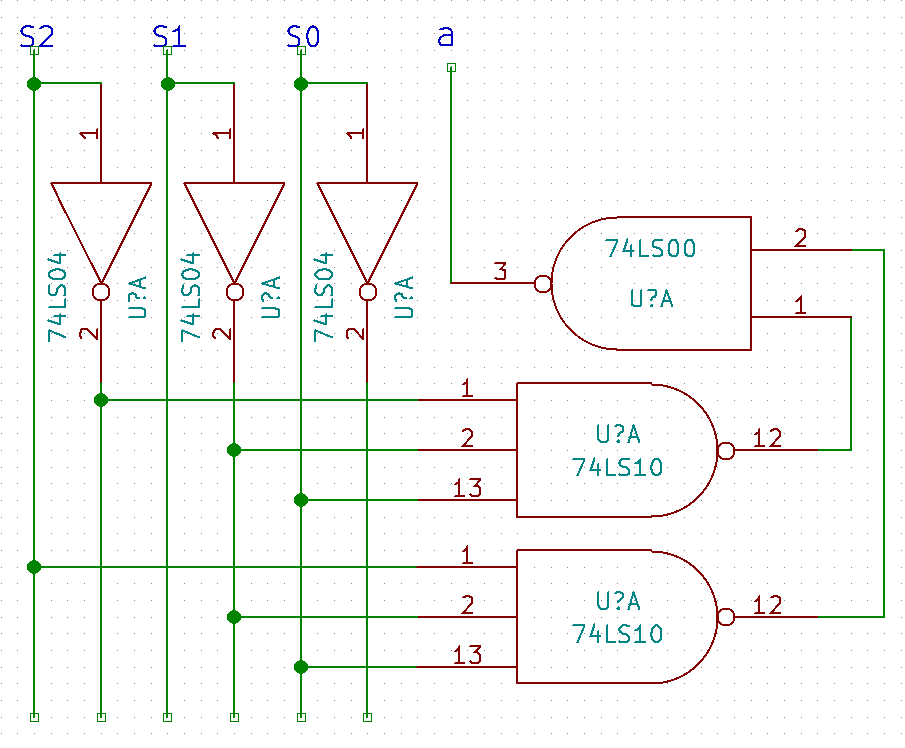
\includegraphics[width=6in]{a.png}
\end{figure}
\begin{figure}[H]
    \centering
    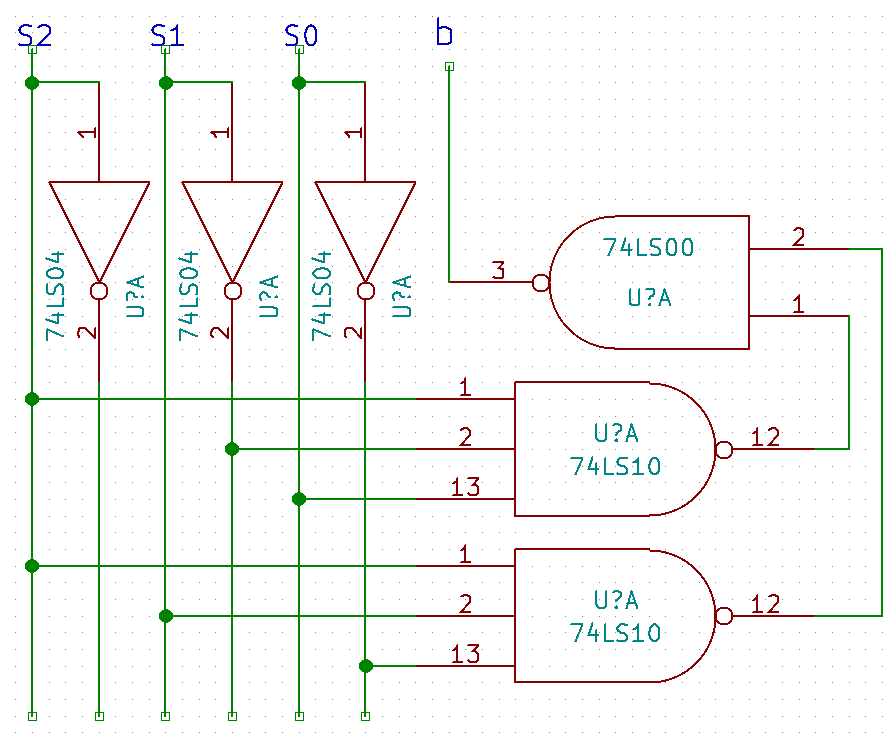
\includegraphics[width=6in]{b.png}
\end{figure}
\begin{figure}[H]
    \centering
    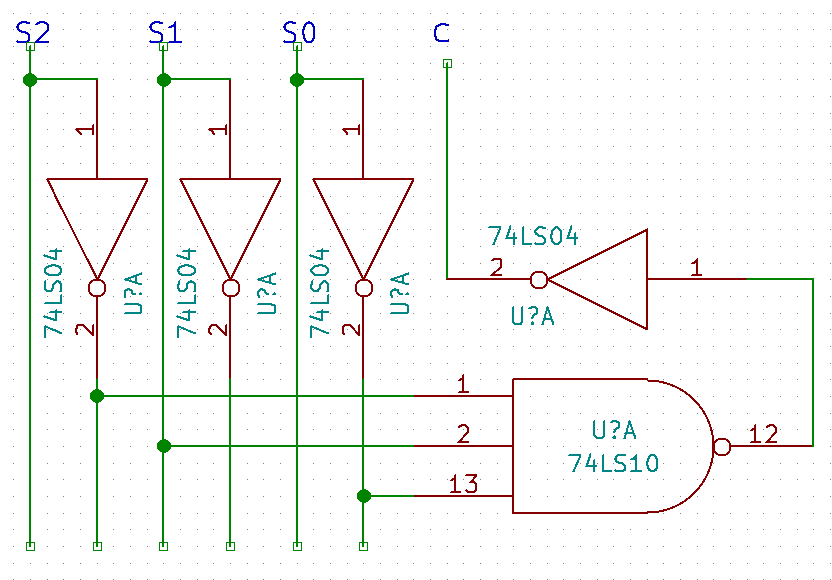
\includegraphics[width=6in]{c.png}
\end{figure}
\begin{figure}[H]
    \centering
    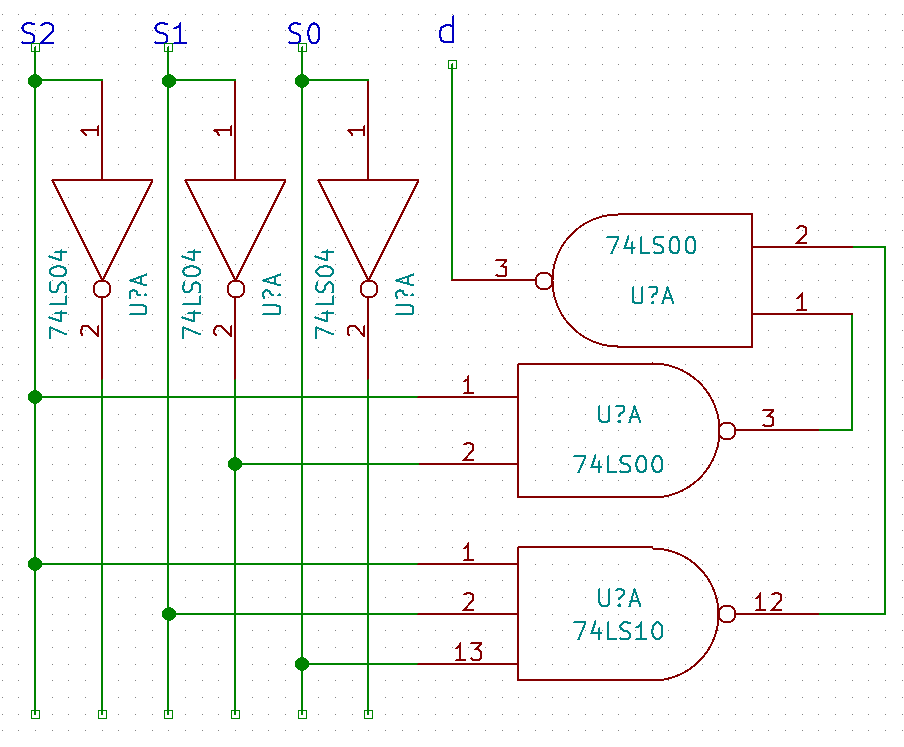
\includegraphics[width=6in]{d.png}
\end{figure}
\begin{figure}[H]
    \centering
    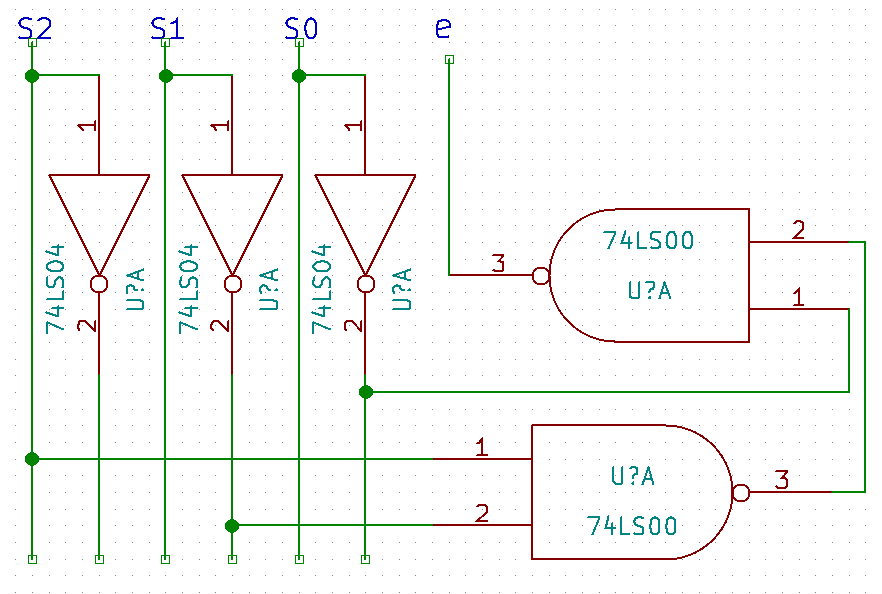
\includegraphics[width=6in]{e.png}
\end{figure}
\begin{figure}[H]
    \centering
    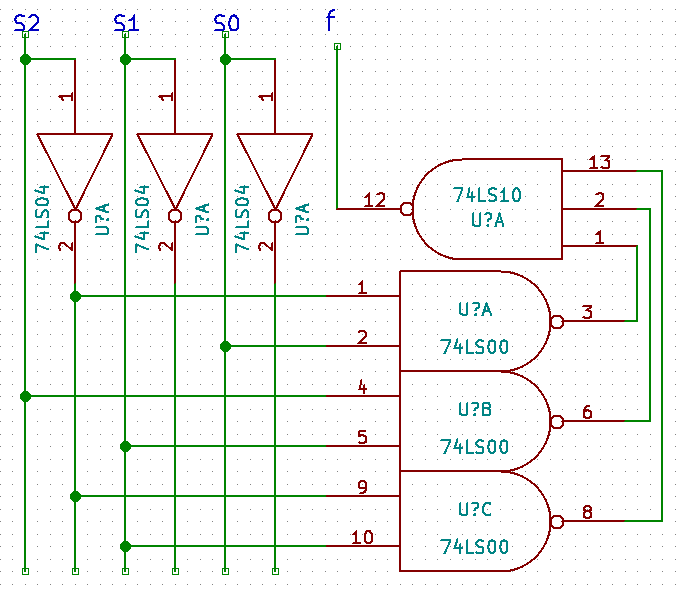
\includegraphics[width=6in]{f.png}
\end{figure}
\begin{figure}[H]
    \centering
    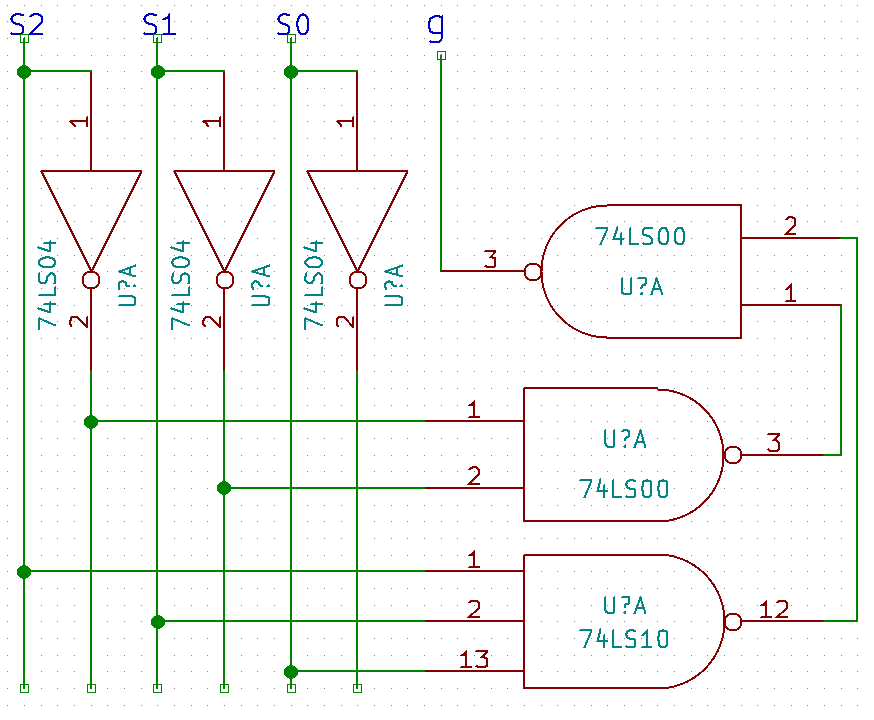
\includegraphics[width=6in]{g.png}
\end{figure}
\subsection{Wiring List}
\begin{tabular}{| C{1.2cm} | C{1.2cm} | C{.5cm} | C{1.2cm} | C{1.2cm} |}
    \hline
    \hline Chip & Pin & to & Chip & Pin \\
    \hline \multicolumn{2}{|c|}{S0} &~& 1 & 1 \\
    \hline \multicolumn{2}{|c|}{S1} &~& 1 & 3 \\
    \hline \multicolumn{2}{|c|}{S2} &~& 1 & 5 \\

    % a
    \hline 1 & 1 &~& 3 & 1 \\
    \hline 1 & 4 &~& 3 & 2 \\
    \hline 1 & 6 &~& 3 & 13 \\

    \hline 1 & 2 &~& 3 & 3 \\
    \hline 3 & 2 &~& 3 & 4 \\
    \hline 1 & 5 &~& 3 & 5 \\

    \hline 3 & 12 &~& 6 & 1 \\
    \hline 3 & 6 &~& 6 & 2 \\

    \hline 6 & 3 &~& \multicolumn{2}{|c|}{a} \\

    % b
    \hline 3 & 1 &~& 3 & 11 \\
    \hline 3 & 4 &~& 3 & 10 \\
    \hline 3 & 5 &~& 3 & 9 \\

    \hline 1 & 2 &~& 4 & 1 \\
    \hline \multicolumn{2}{|c|}{S1} &~& 4 & 2 \\
    \hline \multicolumn{2}{|c|}{S2} &~& 4 & 13 \\

    \hline 3 & 8 &~& 6 & 4 \\
    \hline 4 & 12 &~& 6 & 5 \\

    \hline 6 & 6 &~& \multicolumn{2}{|c|}{b} \\

    % c
    \hline 1 & 2 &~& 4 & 3 \\
    \hline \multicolumn{2}{|c|}{S1} &~& 4 & 4 \\
    \hline 1 & 6 &~& 4 & 5 \\

    \hline 4 & 6 &~& 1 & 13 \\

    \hline 1 & 12 &~& \multicolumn{2}{|c|}{d} \\

    % d
    \hline 1 & 4 &~& 2 & 1 \\
    \hline \multicolumn{2}{|c|}{S2} &~& 2 & 2 \\

    \hline \multicolumn{2}{|c|}{S0} &~& 4 & 11 \\
    \hline \multicolumn{2}{|c|}{S1} &~& 4 & 10 \\
    \hline \multicolumn{2}{|c|}{S2} &~& 4 & 9 \\

    \hline 2 & 3 &~& 6 & 13 \\
    \hline 4 & 8 &~& 6 & 12 \\

    \hline 6 & 11 &~& \multicolumn{2}{|c|}{d} \\

    % e
    \hline 1 & 4 &~& 2 & 4 \\
    \hline \multicolumn{2}{|c|}{S2} &~& 2 & 5 \\

    \hline 1 & 2 &~& 6 & 9 \\
    \hline 2 & 6 &~& 6 & 10 \\

    \hline 6 & 8 &~& \multicolumn{2}{|c|}{e} \\

    % f
    \hline \multicolumn{2}{|c|}{S0} &~& 2 & 13 \\
    \hline 1 & 6 &~& 2 & 12 \\

    \hline \multicolumn{2}{|c|}{S1} &~& 2 & 10 \\
    \hline \multicolumn{2}{|c|}{S2} &~& 2 & 9 \\

    % Out of 2-NAND use 3-NAND
    \hline \multicolumn{2}{|c|}{S1} &~& 5 & 1 \\
    \hline 1 & 6 &~& 5 & 2 \\
    \hline \multicolumn{2}{|c|}{VCC} &~& 5 & 13 \\

    \hline 2 & 11 &~& 5 & 9 \\
    \hline 2 & 8 &~& 5 & 10 \\
    \hline 5 & 12 &~& 5 & 11 \\

    \hline 5 & 8 &~& \multicolumn{2}{|c|}{f} \\

    % g

    % Out of 2-NAND use 3-NAND
    \hline \multicolumn{2}{|c|}{S1} &~& 5 & 1 \\
    \hline 1 & 6 &~& 5 & 2 \\
    \hline \multicolumn{2}{|c|}{VCC} &~& 5 & 13 \\

    \hline
\end{tabular}
\section{References}
Ronald J. Tocci et al. 2011. Digital Systems: Principles and Applications, 11\textsuperscript{th} Ed.

\end{document}
